\chapter{Minimum Spanning Tree - MST}
\paragraph*{INPUT}: Grafo connesso non orientato pesato $G=(V,E)$ con:\\
$W:E \rt R^+$ tale che $W(u,v)$ è il peso dell'arco (u,v).
\paragraph*{OUTPUT}: $T \subseteq E$ aciclico tale che:
\begin{enumerate}
    \item $\forall v \in V, \exists (u,v) \in T$
    \item $W(T) = \sum_{(u,v)\in T} W(u,v)$ è minimo
\end{enumerate}
$G_T = (V,T) \rt$ Minimum Spanning Tree (MST).
\begin{center}
    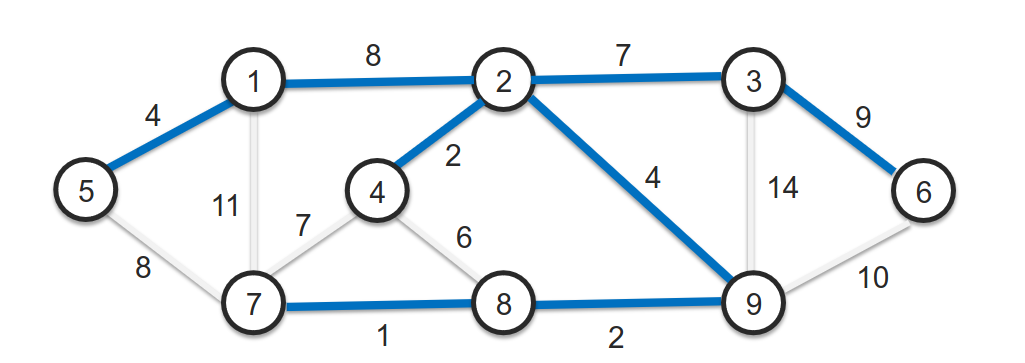
\includegraphics[width=80mm,scale=0.5]{minimum_spanning_tree.png}
\end{center}
$W(T)=37$
\section{Soluzione Generica}
\paragraph*{Algoritmo Generico}
\begin{enumerate}
    \item Inizializza un insieme A vuoto
    \item Aggiunge ad ogni passo un arco (u,v) in modo tale che $A \cup \{(u,v)\}$
    è sottoinsieme dell'insieme T degli archi MST
    \item L'algoritmo termina non appena $A=T$ (cioè, $G_A=(V,T)$ è MST)
\end{enumerate}
$(u,v)$ \ra arco sicuro per A (cioè appartiene a MST)
\begin{lstlisting}[language=Java, escapeinside={@*}{*@}]
    Procedura Generic_MST(G,W)
        A = @*\empt*@
        while @*$G_A = (V,A) \neq$*@ MST do
            trova arco (u,v) sicuro per A
            A = A @*$\cup$*@ {(u,v)}
        return A
\end{lstlisting}
\section{Definizioni Principali}
\subsection{Taglio}
\definizione{Definizione di Taglio: Partizione di V in due insiemi $V'$ e $V-V'$}
\subsection{Arco che Attraversa il Taglio}
\definizione{Definizione di Arco che \underline{Attraversa} il Taglio: arco $(u,v) \in E$ tale che u appartiene a $V'$ e v 
appartiene a $V'-V$} 
\paragraph*{Esempio di Taglio}
\begin{center}
    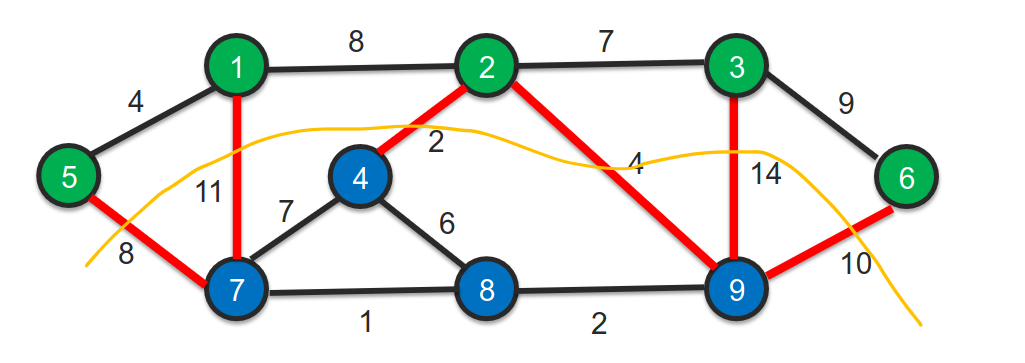
\includegraphics[width=80mm,scale=0.5]{mst_taglio.png}
\end{center}
$V' = \{1,2,3,5,6\}$\\
$V'-V=\{4,7,8,9\}$\\
\subsection{Taglio che rispetta un insieme}
\definizione{Un taglio che \underline{rispetta} un insieme $A \subseteq E$, se nessun arco di A
attraversa il taglio}
\begin{center}
    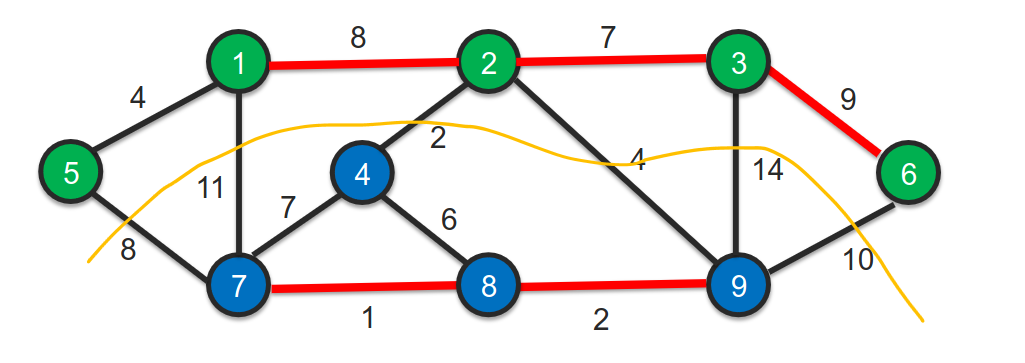
\includegraphics[width=80mm,scale=0.5]{mst_taglio_rispetta.png}
\end{center}
Il taglio rispetta $A = \{(1,2),(2,3),(3,6),(7,8),(8,9)\}$.
\subsection{Arco Leggero}
\definizione{Arco di peso minimo che attraversa il taglio}
\begin{center}
    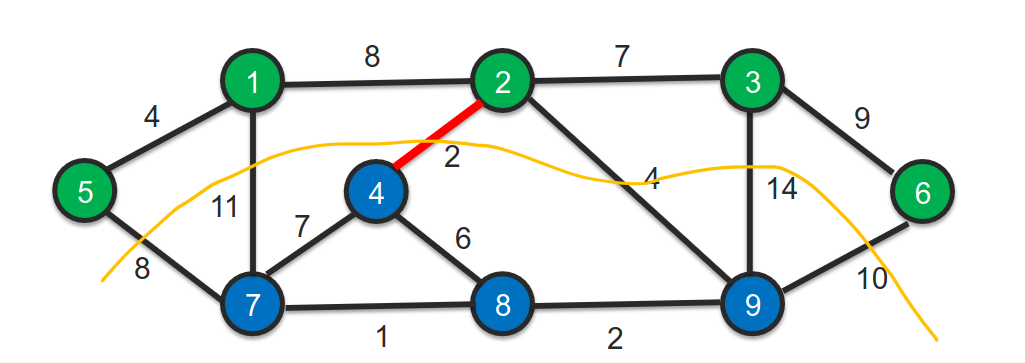
\includegraphics[width=80mm,scale=0.5]{mst_taglio_leggero.png}
\end{center}
(4,2) \ra arco \underline{leggero}
\section{Teorema dell'arco sicuro}
Dati un grafo connesso non orientato e pesato $G=(V,E)$, un sottoinsieme A dell'insieme T di archi di un
Minimum Spanning Tree (MST) e un qualsiasi taglio che rispetti A, allora un arco leggero (u,v) del taglio è
sicuro per A, cioè $A \cup \{(u,v)\} \subseteq T$.
\subsection{Proof}
Considero T \ra insieme di archi di un MST.\\
$A \subseteq T \rt$ sottoinsieme di T.\\
Taglio che rispetta A = (\tikz \fill[green] (0,0) circle (2pt);, \tikz \fill[blue] (0,0) circle (2pt);).\\
$(u,v) \rt$ arco leggero del taglio.
\begin{center}
    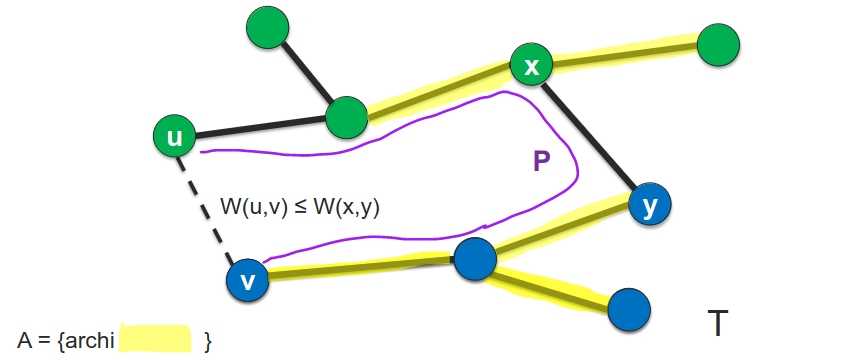
\includegraphics[width=80mm,scale=0.5]{arco_sicuro_dim_mst.png}
\end{center}
Il peso $W(u,v)$ è sicuramente $\leq$ rispetto al peso $W(x,y)$.\\
Sostituisco $(x,y)$, con $(u,v)$ e inserisco quindi l'arco $(u,v)$ all'interno
del grafo e noto che il grafo resta comunque un albero, vedo che resta un MST dato
che non ci sono cicli, ottengo quindi $T'$ con $W(T') \leq W(T)$.\\
\begin{center}
    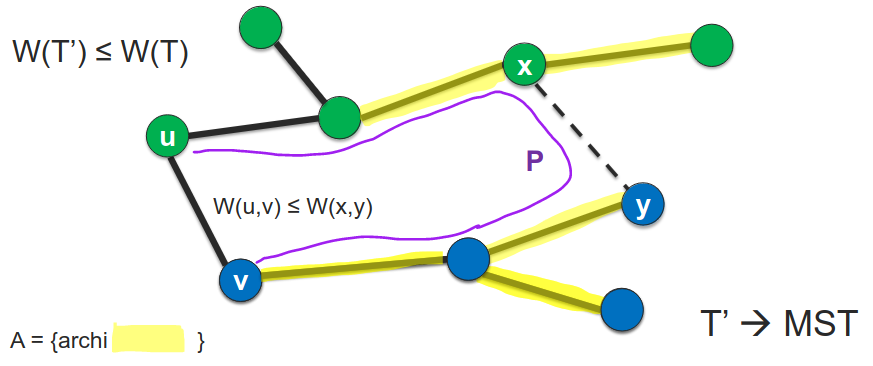
\includegraphics[width=80mm,scale=0.5]{arco_sicuro_dim_mst_2.png}
\end{center}
Per ipotesi, $A \subseteq T$ non contiene $(u,v)$ e $(x,y)$ e per costruzione $T'$ 
non contiene $(x,y)$.\\
$\implies A \subseteq T'$\\
$A \cup \{(u,v)\} \subseteq T'$
%Arrivato a slide 40